\documentclass{article}% insert '[draft]' option to show overfull boxes
\usepackage{amsmath,amsfonts,amssymb}
\usepackage{graphicx}
\usepackage{epstopdf}
\usepackage{subfigure}
\usepackage{float} 
\usepackage{hyperref}  % for urls and hyperlinks


\newcommand{\BigO}[1]{\ensuremath{\operatorname{O}\bigl(#1\bigr)}}
\usepackage[left = 1in, right = 1in, top=1in, bottom=1in]{geometry}
{\setlength{\parindent}{0cm}
\numberwithin{equation}{section}

\title{Convergence of Fixed Geometry Nozzles Using the Pseudo-1D Euler Equations}
\author{Alex Le $\&$ Christopher Uyeda}

\begin{document}

\maketitle

\section{Introduction}
The pseudo-1D Euler equations will be explored for the case of an unsteady nozzle problem with fixed geometry. The simulations of the nozzle will be run until the steady state is reached for various pressure ratios that will result in purely subsonic flow, choked subsonic flow, and purely supersonic flow. In each case, the steady state results will be compared to the theoretical shock locations, if they exist, for different nozzles. Because the pseudo-1D Euler equations inherently contain a source terms, fractional splitting methods will be used to account for the source term. The fractional splitting method involves advecting using the Roe approximate Riemann solver, and then updating to the next time step by solving an ODE to account for the source terms.


\section{Physical Model}
The simulation will be modeling flow through a converging-diverging nozzle with two different geometry nozzles given by

\begin{equation}
\begin{split}
r = 1-0.4(1 + cos(\pi(x -16)/8))   \\
\& \\
r = 0.75 - 0.25 \text{sin}(\pi(x - 10)/10)  \\
A = \pi r^2
\end{split}
\end{equation}

which are shown in Fig. \ref{nozzgeo} where Nozzle 1 has $\frac{A}{A_t} = 25$ and Nozzle 2 has $\frac{A}{A_t} = 4$

\pagebreak
\begin{figure}[h!]
\centering
\subfigure[Nozzle 1]{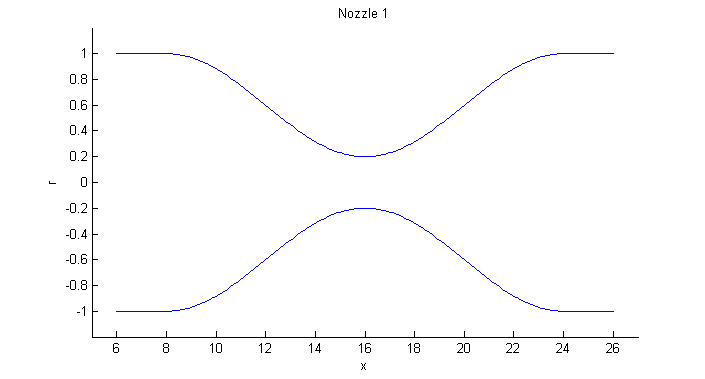
\includegraphics[width=10cm]{nozz1.png}}
\vfill
\subfigure[Nozzle 2]{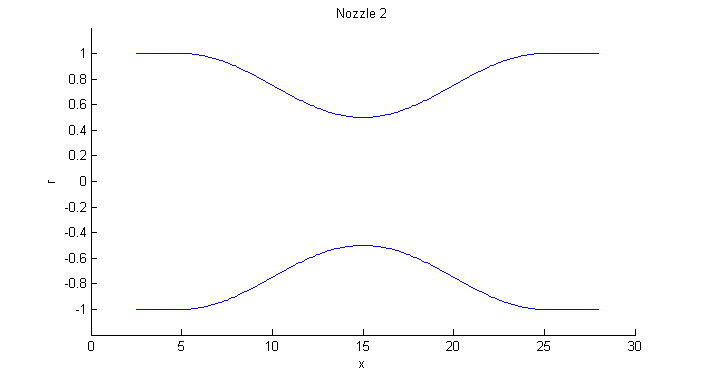
\includegraphics[width=10cm]{nozz2.png}}
\caption{Two different nozzle geometries used in the simulations. \label{nozzgeo}}
\end{figure}

There can be three different types of flow that exist in this nozzle that are dependent on the pressures at the inlet, opened to a pressure reservoir, and the outlet, opened to atmosphere. It is best to define these flow types by the Mach number

\begin{equation}
M = \frac{u}{c}
\end{equation} 
where $ u $ is the velocity and $ c  $ is the speed of sound. The first type of flow results when the pressure ratio, $p_{out} / p_{in}$, is higher than a certain threshold such that the flow is purely subsonic flow, $M < 1$. Flow accelerates through the converging part, but never reaches a sonic speed, or $M = 1$, at the throat of the nozzle. This forces the flow to decelerate through the remaining diverging part of the nozzle such that the flow in the nozzle is entirely subsonic, $M < 1$. The second type of flow is supersonic when the pressure ratio is lower than a certain threshold, where flow accelerates through the converging section and reaches $M = 1$ at the throat. Physics dictates that the flow must now accelerate in the remaining diverging part of the nozzle which results in $M > 1$ at the outlet of the nozzle. These two conditions are a result of the pressure ratios being above a threshold for pure subsonic and below a threshold for supersonic. If the pressure ratio lies in between these thresholds, a shock will form. This type of flow will be considered the choked subsonic flow where the flow reaches sonic at the throat, but a shock appears in the diverging section of the nozzle. The shock exists to raise the pressure of the flow such that it equals the atmospheric pressure at the exit.

\section{Pseudo-1D Euler Equations}
The governing pseudo-1D Euler equation for the simulations is defined by

\begin{equation}
\frac{d}{dt} \left[ \begin{array}{c} \rho A \\ \rho u A \\ e A \end{array} \right] + \frac{d}{dx} \left[ \begin{array}{c} \rho u A \\ (\rho u^2 + p) A \\ u(e + p)A \end{array} \right] = \left[ \begin{array}{c} 0 \\ p \frac{dA}{dx} \\ 0 \end{array} \right] \label{psuedoeuler}
\end{equation}

where the area can be pulled out by

\begin{equation*}
\begin{split}
A q_t + f(A q)_x = S \\
A q_t + \frac{dA}{dx} f(q) + A f(q)_x = S \\
q_t + f(q)_x = \frac{1}{A}S - \frac{1}{A} \frac{dA}{dx} f(q) \\
\end{split}
\end{equation*}

where S is the original source term vector. The reformulated equation then becomes 

\begin{equation}
\frac{d}{dt} \left[ \begin{array}{c} \rho  \\ \rho u  \\ e \end{array} \right] + \frac{d}{dx} \left[ \begin{array}{c} \rho u  \\ \rho u^2 + p \\ u(e + p) \end{array} \right] = \left[ \begin{array}{c} -\frac{1}{A}\frac{dA}{dx} \rho u \\ -\frac{1}{A} \frac{dA}{dx} \rho u^2  \\ -\frac{1}{A} \frac{dA}{dx}  u(e + p) \end{array} \right]
\end{equation}

 where the new conserved variables are $q = [\rho, \rho u, e]^T$, similar to the 1D Euler equations, which makes implementation with existing Riemann solvers much easier. 

\section{Boundary Conditions}
In order to initiate flow through the nozzle, boundary conditions must be used at the inlet and outlet. The proper implementation of these conditions are crucial to avoid artificial reflections at the inlet or outlet. Both boundary conditions are purely driven by defined pressures.

\subsection{Subsonic Inlet}
In the case of a subsonic inlet, the 1-wave is traveling out of the domain while the 2-wave and 3-wave are moving into the domain. This means that two primitive variables must be defined from the boundary, $u_0$ and $p_0$ in the first ghost cell. Because pressure will be defined at the inlet from the reservoir, the corresponding $u_0$ can be determined by the Hugoniot-Loci for the 3-wave that links $q_r$ to $q_0$, where $q_0$ are the conserved variables in the first ghost cell. The Rankine-Hugoniot conditions are applied in this case to derive an equation for $u_0$ in terms of $p_0$ and $\gamma$ [1]

\begin{equation}
u_0 = u_1 - \frac{2}{\sqrt{2 \gamma (\gamma - 1)}} \sqrt{\frac{\gamma p_1}{\rho_1}} \left( \frac{1 - p_0 / p_1}{\sqrt{1 + \beta p_0 / p_1}} \right)
\end{equation}

where $\beta = (\gamma + 1) / (\gamma  - 1)$ and the subscript 1 refers to the first interior cell. The corresponding density is then defined as

\begin{equation}
\rho_0 = \left( \frac{1 + \beta p_0 / p_1}{p_0 /p_1 + \beta} \right) \rho_1
\end{equation}

The energy is defined by 

\begin{equation}
e = \frac{p}{\gamma - 1} + \frac{1}{2} \rho u^2
\end{equation}

so the resulting conserved variables at the first ghost cell is 

\begin{equation}
q_0 =  \left[ \begin{array}{c} \rho_0 \\ \rho_0 u_0 \\ \frac{p_0}{\gamma - 1} + \frac{1}{2} \rho_0 u_0^2 \end{array} \right]
\end{equation}

where $q_j(i)$ refers to the ith component of q at the jth cell.

\subsection{Subsonic Outlet}
The subsonic outlet is similar to the subsonic inlet, but now the 1 wave is traveling into the domain while the 2-wave and 3-wave are moving out of the domain. In this case, only one primitive variable must be defined from the boundary, $p_{atm}$, but in order to satisfy the Riemann condition for the Roe solver, density and momentum are also defined along the 1-wave. The corresponding velocity is 

\begin{equation}
u_{N+1} = u_N + \frac{2}{\sqrt{2 \gamma (\gamma - 1)}} \sqrt{\frac{\gamma p_N}{\rho_N}} \left( \frac{1 - p_{atm} / p_N}{\sqrt{1 + \beta p_{atm} / p_N}} \right)
\end{equation}

where N refers to the last cell in the interior and N $+$ 1 is the first ghost cell. The corresponding density on the 1-wave is

\begin{equation}
\rho_{N+1} = \left( \frac{1 + \beta p_{atm} / p_N}{p_{atm} /p_N + \beta} \right) \rho_N
\end{equation}

Thus the resulting conserved variables defined at the first ghost cell at the outlet, $q_n$, is

\begin{equation}
q_n =  \left[ \begin{array}{c} \rho_{N+1} \\ \rho_{N+1} u_{N+1} \\ \frac{p_{atm}}{\gamma - 1} + \frac{1}{2} \rho_{N+1} u_{N+1}^2 \end{array} \right]
\end{equation}

\subsection{Supersonic Outlet}
For the supersonic outlet, all the waves are now traveling out of the domain. This means the conserved variables at the first ghost cell at the outlet, $q_n$, is easily defined by an extrapolation 

\begin{equation}
q_n  =  q_{n-1}
\end{equation}

\section{Numerical Method}
\subsection{Riemann Problem - Euler Equations}
To solve the Euler equation Riemann problem, the waves are split into the left going and right going waves according to the eigenvalues. This means that if the flow is subsonic then $\lambda^1$ is a left going wave and $\lambda^2$ and $\lambda^3$ are right going waves, while if the flow is supersonic then all waves are right going waves. The flux Jacobian of the system is given by

\begin{equation}
f'(q) = \left[ \begin{array}{ccc} 0 & 1 & 0 \\ p_{\rho} - u^2 &  u(2 - p_e) &  p_e \\  u(p_\rho - H) & H - u^2 p_e  &  u(1 + p_e) \end{array} \right] \label{1deulerjacobian}
\end{equation}

where $H = \frac{e + p}{\rho}$, $p_\rho = \frac{\gamma - 1}{2} u^2 $, and $p_e = \gamma - 1$. The eigenvalues may be solved by taking the determinant and setting it equal to zero

\begin{equation}
det \left[ \begin{array}{ccc} -\lambda & 1 & 0 \\ p_{\rho} - u^2 &  u(2 - p_e) - \lambda &  p_e \\  u(p_\rho - H) & H - u^2 p_e  &  u(1 + p_e) - \lambda \end{array} \right] = 0
\end{equation}

where the eigenvalues are then given by 

\begin{equation}
\lambda^1 = u - c,  \ \ \lambda^2 =u , \ \ \lambda^3 = u + c \label{eigval}
\end{equation}

Solving for the eigenvectors, r, results in

\begin{equation}
\begin{split}
(f'(q) - \lambda I) r = 0 \\
R = \left[ \begin{array}{c |c | c} r^1 & r^2 & r^3 \end{array} \right]= \left[ \begin{array}{ccc} 1 & 1 & 1 \\ u- c & u  & u + c \\ H - u c &  H - \frac{c^2}{\gamma - 1} & H + u c   \end{array} \right] 
\end{split}
\end{equation}The coefficients of these eigenvectors, $\alpha$, may be determined by the following which involves taking the inverse of the eigenvector matrix, R.

\begin{equation}
q_r - q_l = R \alpha \rightarrow R^{-1} (q_r - q_l) = \alpha \label{alphaeqn}
\end{equation}

where 

\begin{equation}
\begin{split}
R^{-1} = \left[ \begin{array}{ccc} \frac{c^2 + H (\gamma-1) + c u + (\gamma-1) u^2}{2 c^2} & -\frac{c + (\gamma - 1) u}{2 c^2} & \frac{\gamma - 1}{2 c^2} \\ \frac{ (\gamma - 1) (H - u^2)}{c^2} & \frac{(\gamma - 1) u}{c^2} & - \frac{\gamma - 1}{c^2} \\   \frac{c^2 - H (\gamma - 1) - c u + (\gamma - 1) u^2}{2 c^2} & \frac{c - (\gamma - 1) u}{2 c^2} & \frac{\gamma - 1}{2 c^2} \end{array} \right] \\ 
%= \left[ \begin{array}{ccc} \frac{e (1 - \gamma) + p (1 - \gamma) + \rho(c^2 + c u + (\gamma - 1) u^2)}{2 c^2 \rho} & -\frac{u(\gamma - 1) + c}{2 c^2} & \frac{\gamma - 1}{2 c^2}   \\ \frac{(\gamma - 1)(e + p - \rho u^2)}{c^2 \rho} & \frac{u (\gamma - 1)}{c^2} & -\frac{\gamma - 1}{c^2} \\ \frac{e (1 - \gamma) + p (1 - \gamma) + \rho(c^2 - c u + (\gamma - 1)u^2)}{2 c^2 \rho} & \frac{c - u(\gamma - 1)}{2 c^2} & \frac{\gamma - 1}{2 c^2}  \end{array} \right]
\end{split}
\end{equation}


The coefficients may then be solved to be

\begin{equation}
\begin{split}
\alpha = R^{-1}(qr - ql)  = R^{-1} \delta \\
%=  \left[ \begin{array}{c} \frac{e (1 - \gamma) + p (1 - \gamma) + \rho(c^2 + c u + (\gamma - 1) u^2)}{2 c^2 \rho} \delta^1  - \frac{u(\gamma - 1) + c}{2 c^2} \delta^2 +\frac{\gamma - 1}{2 c^2} \delta^3 \\ \frac{(\gamma - 1)(e + p - \rho u^2)}{c^2 \rho} \delta^1 + \frac{u (\gamma - 1)}{c^2} \delta^2  -\frac{\gamma - 1}{c^2} \delta^3 \\ \frac{e (1 - \gamma) + p (1 - \gamma) + \rho(c^2 - c u + (\gamma - 1)u^2)}{2 c^2 \rho} \delta^1 + \frac{c - u(\gamma - 1)}{2 c^2} \delta^2 +  \frac{\gamma - 1}{2 c^2} \delta^3 \end{array} \right] \\
= \left[ \begin{array}{c} \frac{c^2 + H (\gamma-1) + c u + (\gamma-1) u^2}{2 c^2} \delta^1 -\frac{c + (\gamma - 1) u}{2 c^2} \delta^2 +   \frac{\gamma - 1}{2 c^2} \delta^3 \\ \frac{ (\gamma - 1) (H - u^2)}{c^2} \delta^1 +  \frac{(\gamma - 1) u}{c^2} \delta^2 -  \frac{\gamma - 1}{ c^2}  \delta^3 \\ \frac{c^2 - H (\gamma - 1) - c u + (\gamma - 1) u^2}{2 c^2} \delta^1 + \frac{c - (\gamma - 1) u}{2 c^2} \delta^2 +   \frac{\gamma - 1}{2 c^2} \delta^3 \end{array} \right] \\
= \left[ \begin{array}{c} (\gamma - 1) \frac{(H + u^2) \delta^1 - u \delta^2 + \delta^3}{2 c^2} + \frac{(c^2 + c u) \delta^1 - c \delta^2}{2 c^2} \\ (\gamma - 1) \frac{(H - u^2)\delta^1 + u \delta^2 - \delta^3}{ c^2} \\ (\gamma - 1) \frac{(u^2 - H) \delta^1 - u \delta^2 + \delta^3}{2 c^2} + \frac{(c^2 - c u) \delta^1 + c \delta^2}{2 c^2} \end{array} \right]
\end{split} \label{coeffcients}
\end{equation}

where $\delta^i$ refers to the ith element of the $\delta = q_r - q_l $ vector. Because solving the exact Riemann solution is very expensive, the Roe approximation is used instead which estimates velocity, $\hat{u}$, total specific enthalpy, $\hat{H}$, and sound speed, $\hat{c}$ [1], by

\begin{equation}
\begin{split}
\hat{u}= \frac{\sqrt{\rho_{i - 1}} u_{i-1} + \sqrt{\rho_i} u_i}{\sqrt{\rho_{i-1}} + \sqrt{\rho_i}}  \\
\hat{H} = \frac{\sqrt{\rho_{i - 1}} H_{i-1} + \sqrt{\rho_i} H_i}{\sqrt{\rho_{i-1}} + \sqrt{\rho_i}} = \frac{(E_{i-1} + p_{i-1})/\sqrt{\rho_{i - 1}}+ (E_i + p_i) / \sqrt{\rho_i} }{\sqrt{\rho_{i-1}} + \sqrt{\rho_i}} \\
\hat{c} = \sqrt{(\gamma - 1) \left( \hat{H} - \frac{1}{2} \hat{u}^2 \right)}
\end{split}
\end{equation}

These values are then plugged into Eqn. \ref{eigval} and \ref{coeffcients} to solve the Riemann problem with the approximated values.

\subsection{Fractional Splitting}
Because the psuedo-1D Euler equation given by Eqn. \ref{psuedoeuler} contains a source term, $p \frac{dA}{dx}$, the typical Riemann solving method can't be applied. In order to account for this source term, a fractional splitting method is incorporated, which is chosen to be the Godunov splitting.
\\
\\
Starting with Gudonov splitting, at each timestep, the solution will be advected and then reacted. This two step method takes the form of

\begin{equation}
\begin{split}
\text{Step 1:} \ \ q_t + \bar{u} q_x = 0 \\
\text{Step 2:} \ \ q_t = \psi(q)
\end{split}
\end{equation}  

The first step will be solved first using the MC limiter method and the second step will be solved by using a two stage Runge-Kutta method to solve the ODE. The two steps when specified to the psuedo-1D Euler equations is given by

\begin{equation}
\begin{split}
\text{Step 1:} \ \ \left[ \begin{array}{c} \rho  \\ \rho u  \\ e \end{array} \right]_t +  \left[ \begin{array}{c} \rho u  \\ \rho u^2 + p \\ u(e + p) \end{array} \right]_x =  0 \\
\text{Step 2:} \ \ \left[ \begin{array}{c} \rho  \\ \rho u  \\ e  \end{array} \right]_t = \left[ \begin{array}{c} -\frac{1}{A}\frac{dA}{dx} \rho u \\ -\frac{1}{A} \frac{dA}{dx} \rho u^2  \\ -\frac{1}{A} \frac{dA}{dx}  (e + p)  \end{array} \right]    \end{split}
\label{eq:splitting}
\end{equation}

\subsection{Flux Limiter Methods}
The first step in the split method is implemented as a modification to an existing Riemann solver within Clawpack, called 'rp1\_euler\_with\_efix.f90'. This is a 1D Euler solver has the Roe-averaged quantities and wave solutions already programmed into it. This solver can be used with limiter methods specified by the 'setrun.py' file.

In general, the flux-limiter method is of the form:

\begin{equation}
Q^{n+1}_i=Q^n_i-\nu(Q^n_i-Q^n_{i-1})-\frac{1}{2}\nu(1-\nu)[\phi(\theta^n_{i+1/2})(Q^n_{i+1}-Q^n_i)-\phi(\theta^n_{i-1/2})(Q^n_{i}-Q^n_{i-1})]
\end{equation}
If $ \bar{u} > 0 $, where $ \nu=\frac{\bar{u}\Delta t}{\Delta x} $, and $ \theta^n_{i-1/2}=\frac{\Delta Q^n_{i-3/2}}{\Delta Q^n_{i-1/2}} $.

The following function of $ \theta $ was implemented for its corresponding limiter function.

\begin{align}
\text{MC:} \ \ & \phi(\theta)=max(0,min(1+\theta)/2,2, 2\theta)
\end{align}

\subsection{Source Terms}
The second step implements an optional source function that uses a Runge-Kutta method to solve a set of three ODEs. The Runge-Kutta solver takes the form:
\begin{equation}
\begin{split}
Q^{**}_i=Q^*_i+\frac{\Delta t}{2} \psi (Q^*_i) \\
Q^{n+1}_i=Q^*_i+ \Delta t \psi(Q^{**}_i)
\end{split}
\end{equation}
Here, $ Q^* $ is the conserved quantity vector after advection, and $ \psi(Q^*) $ are the source terms from Eq. \ref{eq:splitting} evaluated using the quantities from the vector $ Q^* $. This solver uses a forward Euler algorithm by approximating the conserved quantity vector at an intermediate state using a half-time step, and then using this midpoint state $ Q^{**} $ in order to update the solution to the next time level using a full time step, with $ \psi(Q^{**}) $ referring to the source terms evaluated using $ Q^{**} $.

\section{Numerical Results}
All simulations were run with a 1000 mesh over a domain size of 0 to 30 to ensure that the cell spacing is consistent in each simulation and used the MC limiter as previously discussed. The following are the results for each simulation.

\subsection{Subsonic}
The results for nozzle 1 and 2 are shown at the steady state for pressure ratio $\frac{p_{atm}}{p_o} = 0.99$ in Fig. \ref{subsonic}. It can be seen that the pressure ratio at the two boundaries are satisfied while Mach is always below 1 throughout the entire nozzle. As expected, the Mach and flow velocity increased through the converging section and decreased through the diverging section which agrees with physics. Also, because nozzle 1 has a higher area ratio, the flow velocity at the throat is expected to have accelerated faster than that of nozzle 2 which can be observed in the results.


\begin{figure}[h!]
\subfigure[Nozzle 1]{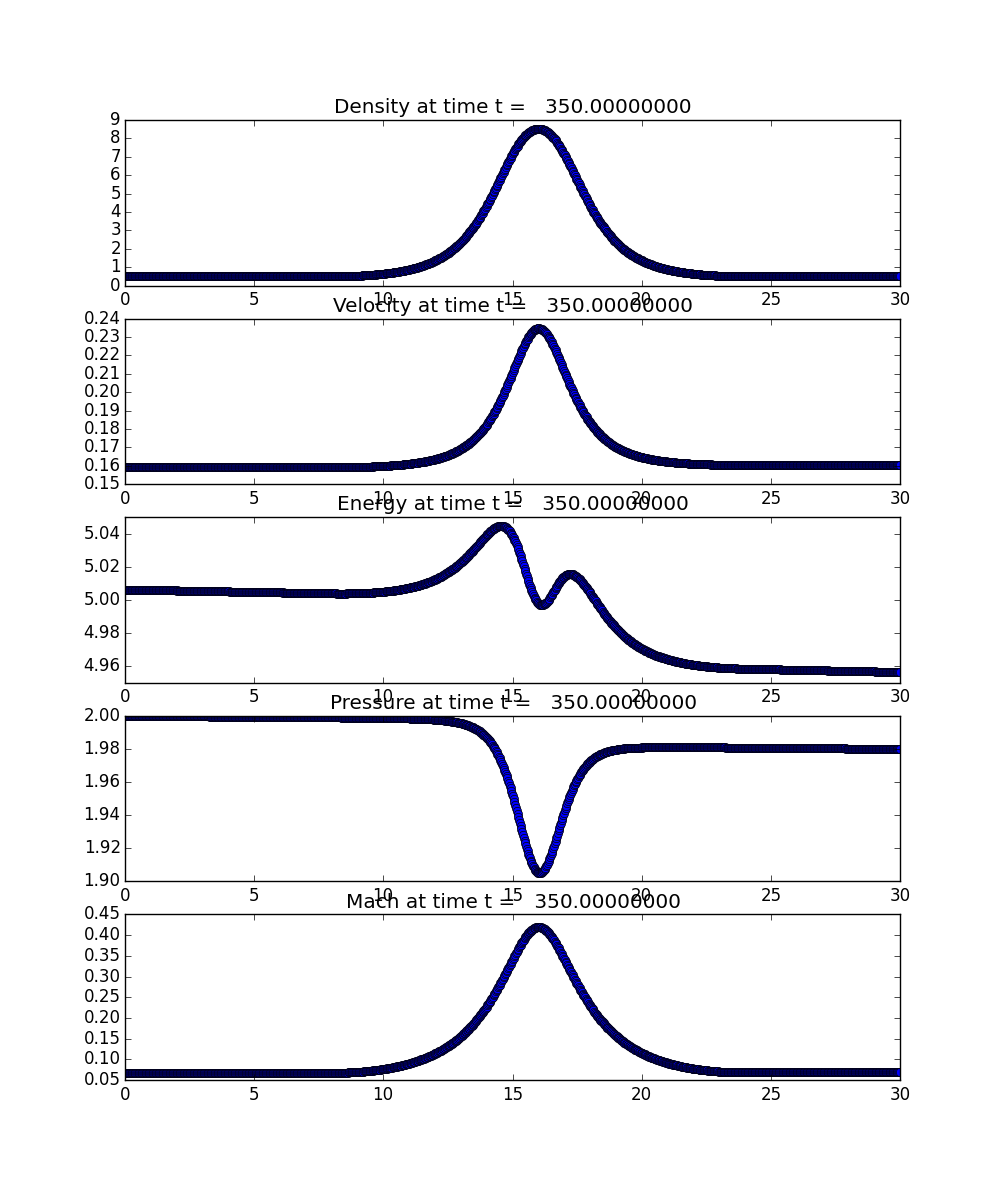
\includegraphics[width=8cm]{nozz1_099.png}}
\subfigure[Nozzle 2]{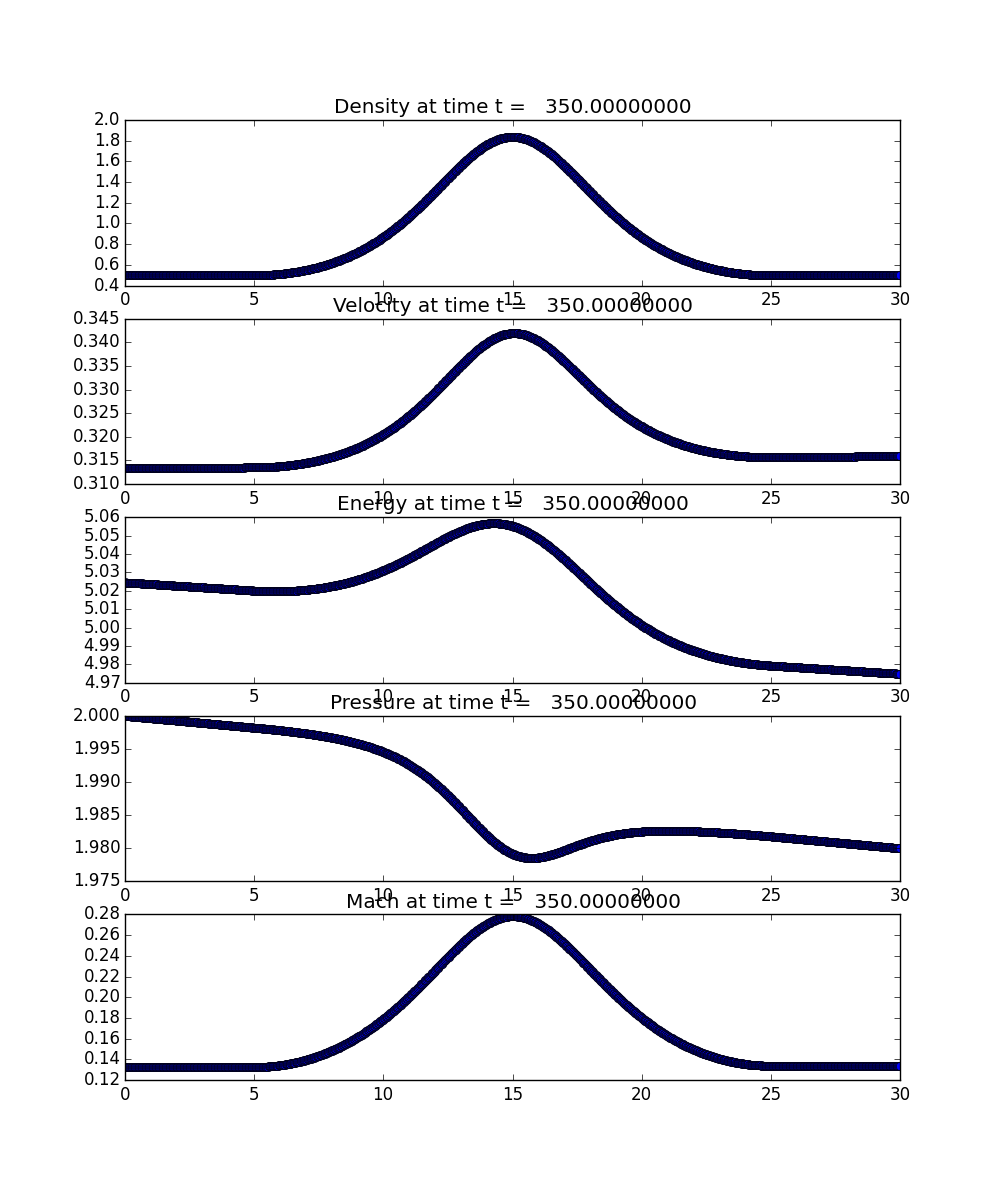
\includegraphics[width=8cm]{nozz2_099.png}}
\caption{a). Nozzle 1 and b). Nozzle 2 converged at steady state for a high pressure ratio which results in subsonic flow. \label{subsonic}}
\end{figure}

\subsection{Choked Subsonic}
The results for nozzle 1 and 2 are shown in Fig. \ref{chokesubsonic} at the steady state for pressure ratio, $\frac{p_{atm}}{p_o}$ = 0.7. The theoretical shock location is calculated and plotted in the Mach plot of the results to compare how well the simulations were able to capture the shock.

\pagebreak

\begin{figure}[h!]
\subfigure[Nozzle 1]{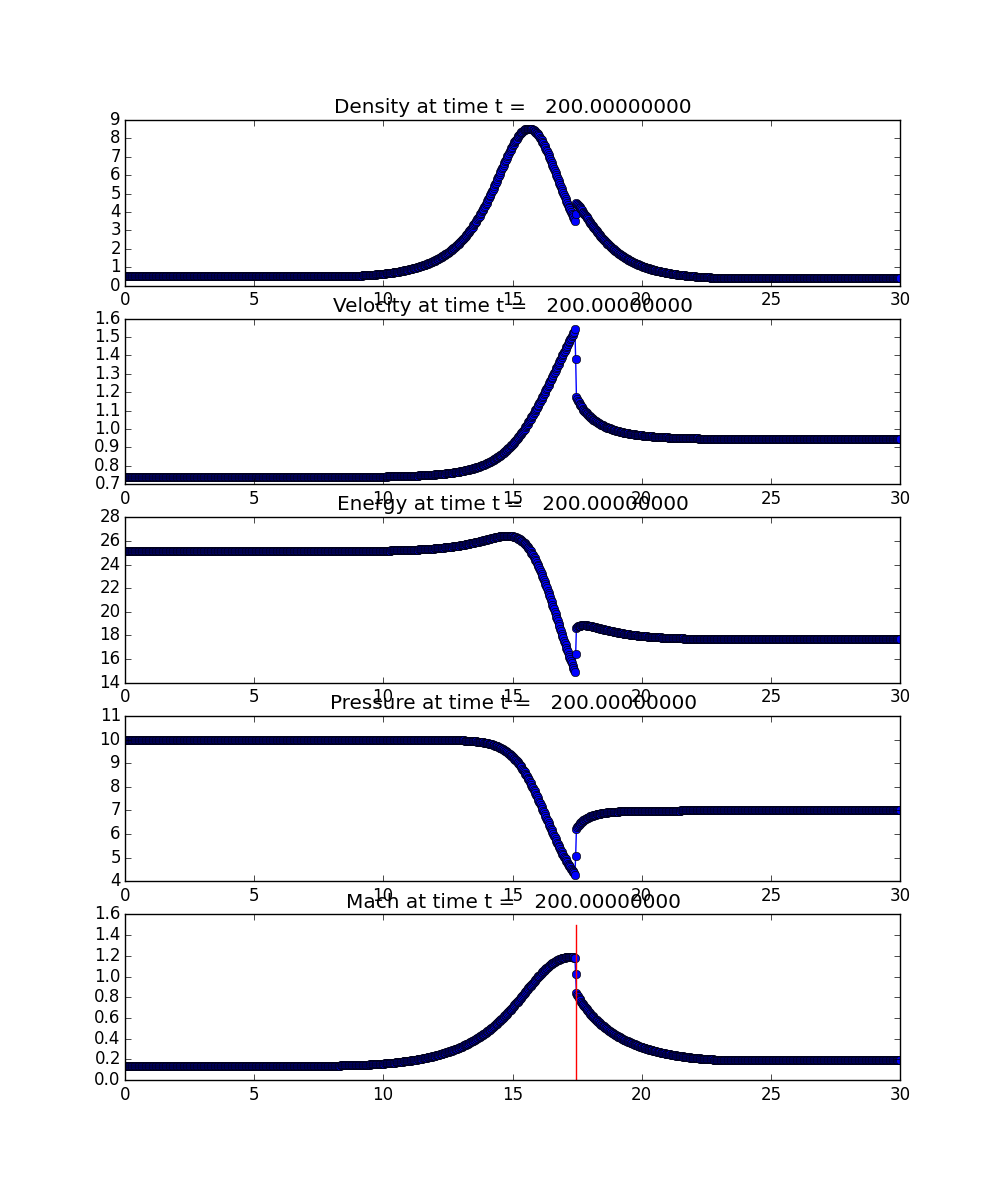
\includegraphics[width=8cm]{nozz1_07.png}}
\subfigure[Nozzle 2]{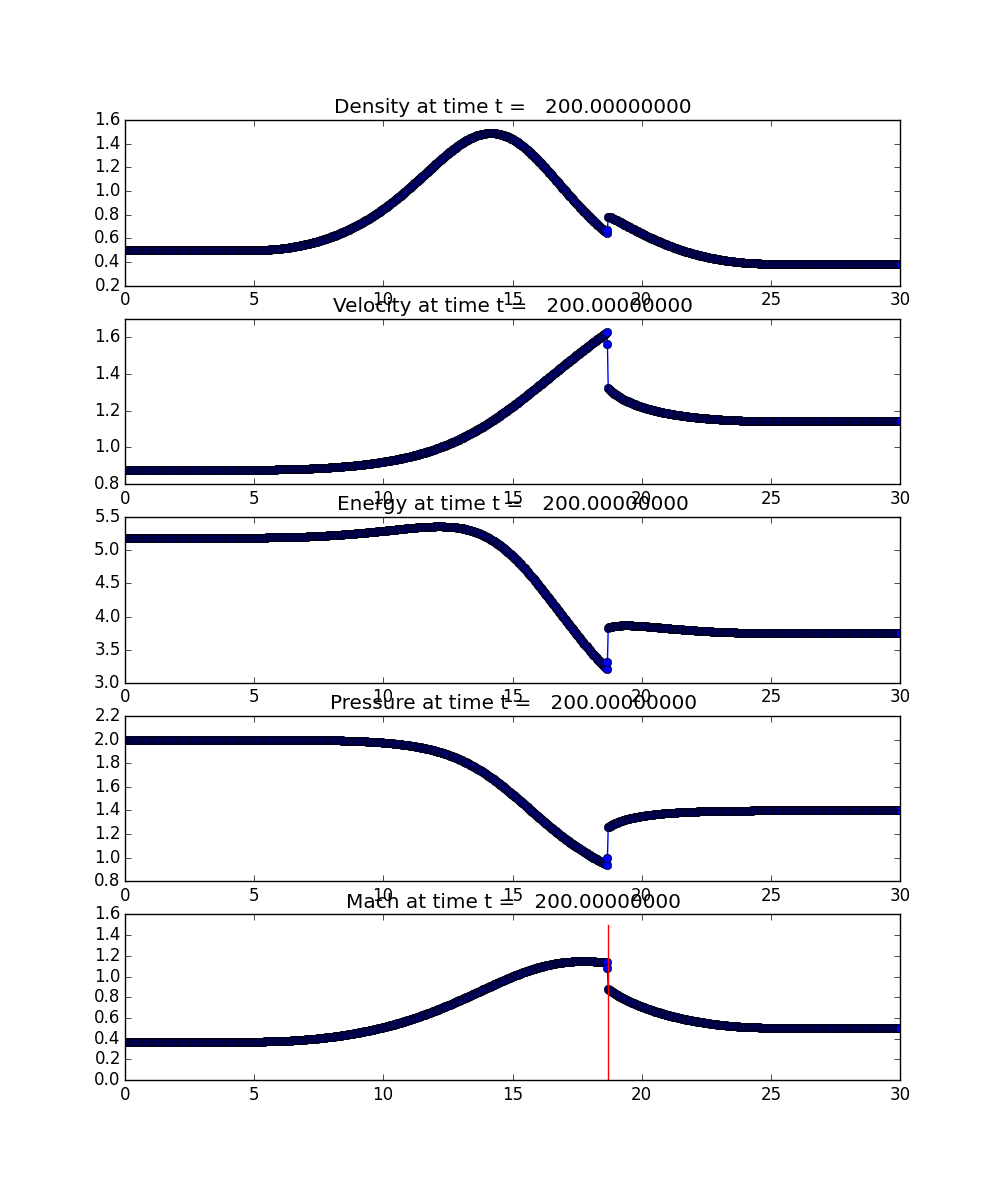
\includegraphics[width=8cm]{nozz2_07.png}}
\caption{a). Nozzle 1 and b). Nozzle 2 converged at steady state for a high pressure ratio which results in choked subsonic flow. \label{chokesubsonic}}
\end{figure}


\subsection{Supersonic}
Unfortunately, the supersonic cases converged to a physically incorrect flow in the nozzle. After the flow becomes sonic at the throat, the flow should continue to accelerate through the diverging section of the nozzle until the constant area section. The simulation shows that the flow instead decreases after the throat and then increases all in the diverging section of the nozzle until the constant area section.

\subsection{Convergence Issues}
Simulations of the two geometry nozzles were able to converge for most cases that had pure subsonic and choked subsonic flows. Special care had to be taken when defining the initial reservoir pressure for each nozzle. It was discovered that a higher reservoir pressure needed to be defined for the higher area ratio nozzle 1 than the other nozzle 2 in order for nozzle 1 to converge properly at lower pressure ratios. For both nozzles, the reservoir pressure needed to be lowered in order to converge for lower pressure ratios that puts the shock close to the nozzle exit, the constant area region, or if the flow should be supersonic throughout the diverging section. Finally, care had to be taken to ensure that the reservoir pressure was not defined to be too low because it was discovered that this led to solutions that blew up.
\\
\\
Even by lowering the reservoir pressure in the cases that the shock approaches the nozzle exit, the steady state simulation put the shocks at incorrect distances when compared to the theoretical solution. This error in the simulations increased as the pressure ratio was lowered, or when the shock got closer to the nozzle exit. Results are shown in Fig. \ref{nozz1shock} and \ref{nozz2shock} where nozzle 2 shows further deviation of the shock location from the theoretical location as the pressure ratio is decreased.

\begin{figure}[h!]
\centering
\subfigure[$\frac{p_{atm}}{p_0}$ = 0.2]{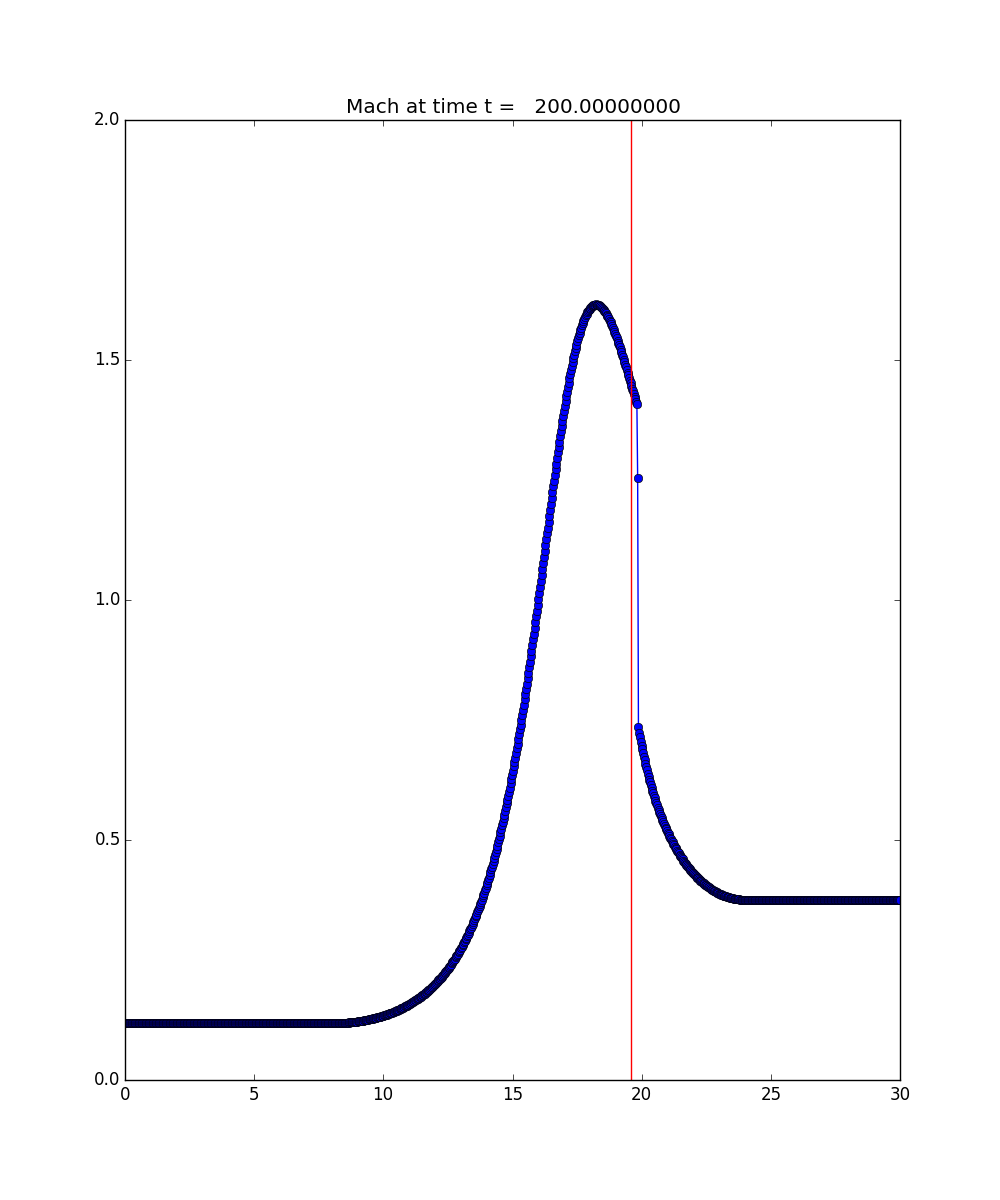
\includegraphics[height=6.5cm]{nozz1_02.png}}
\subfigure[$\frac{p_{atm}}{p_0}$ = 0.15]{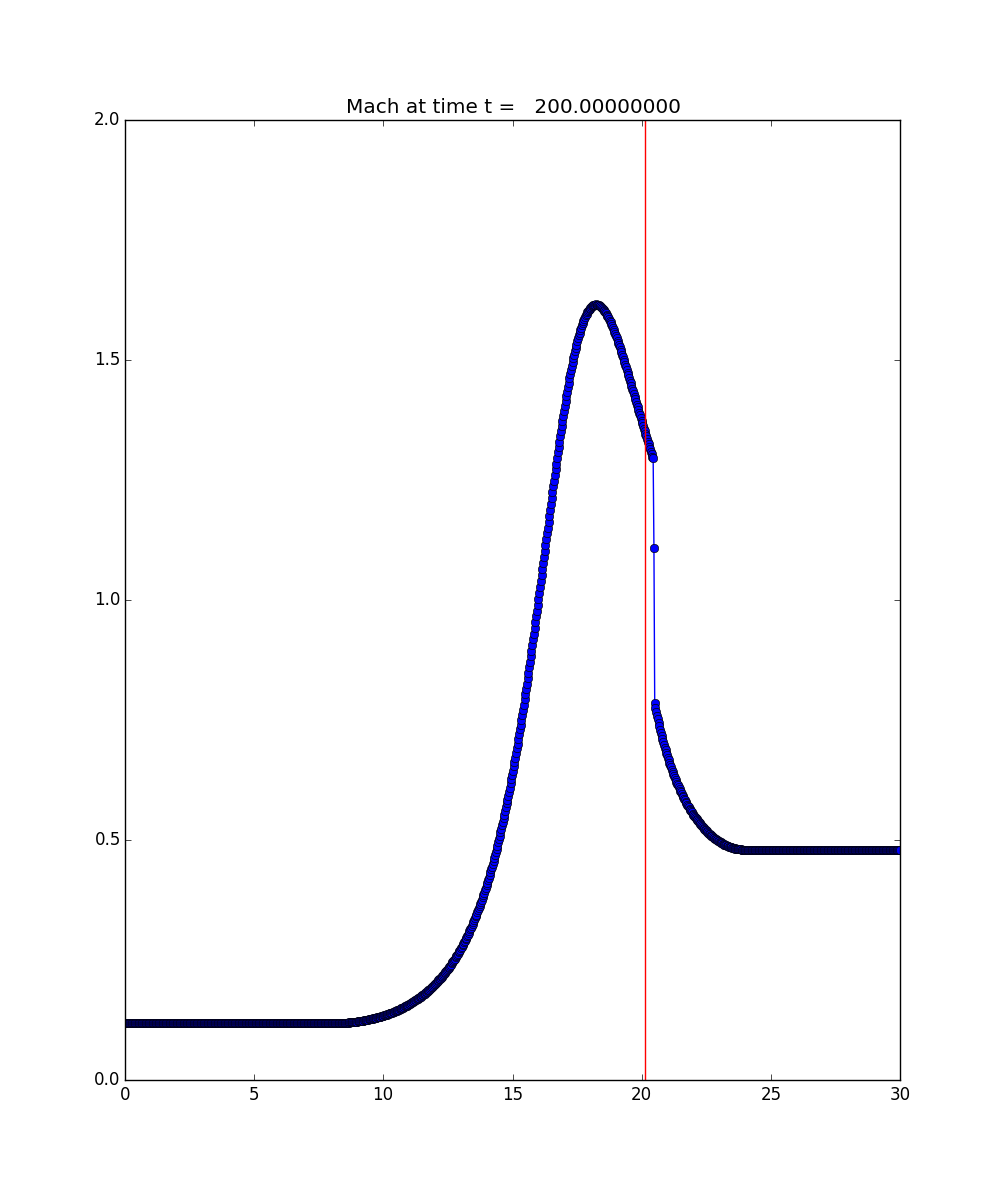
\includegraphics[height=6.5cm]{nozz1_015.png}}
\subfigure[$\frac{p_{atm}}{p_0}$ = 0.1]{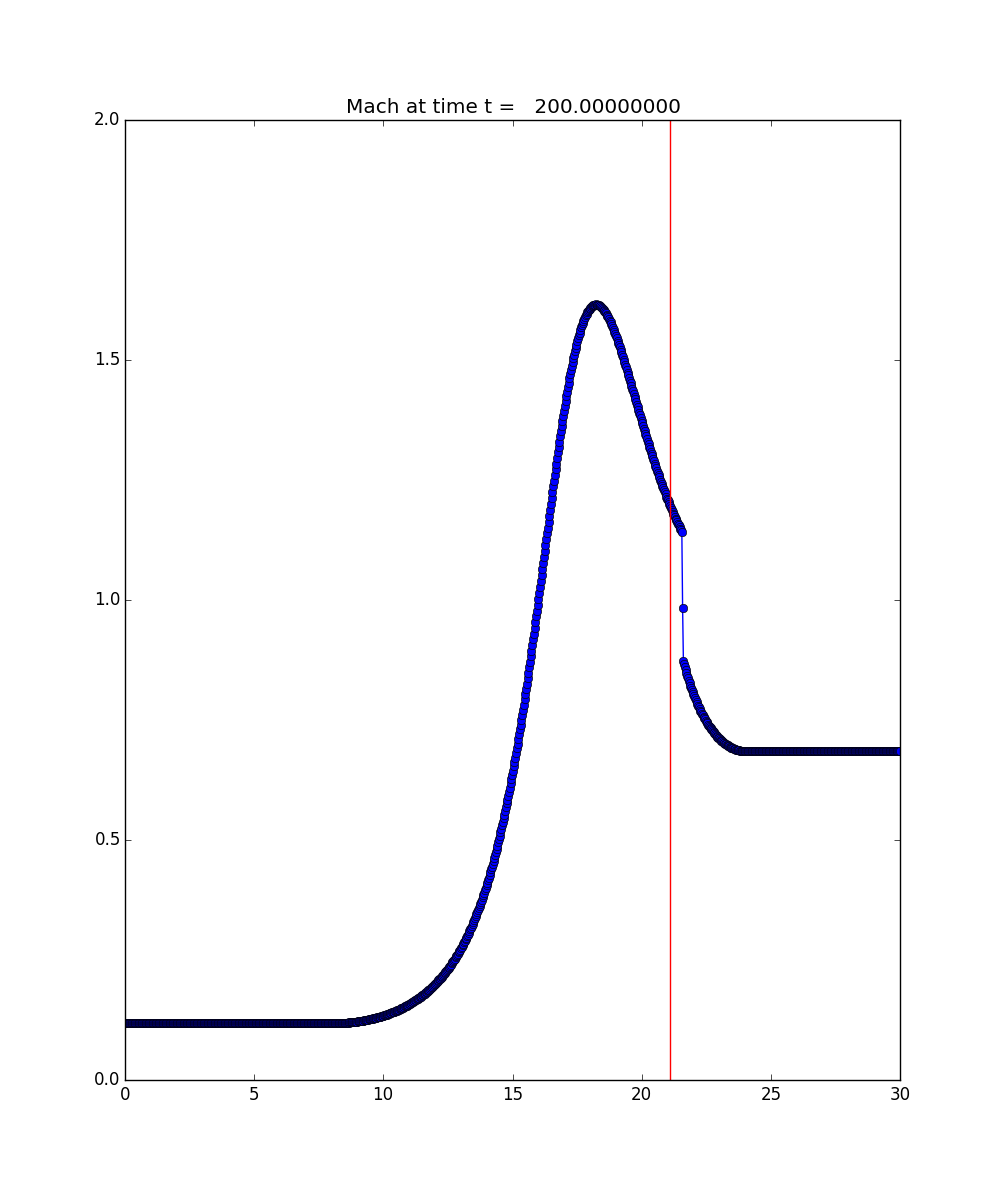
\includegraphics[height=6.5cm]{nozz1_01.png}}
\caption{Mach of Nozzle 1 at steady state for $\frac{p_{atm}}{p_0}$ = a). 0.2, b). 0.15, c). 0.1. As the pressure ratio decreases, the simulation shock deviates further from the theoretical shock location. \label{nozz1shock}}
\end{figure}

\begin{figure}[h!]
\centering
\subfigure[$\frac{p_{atm}}{p_0}$ = 0.45]{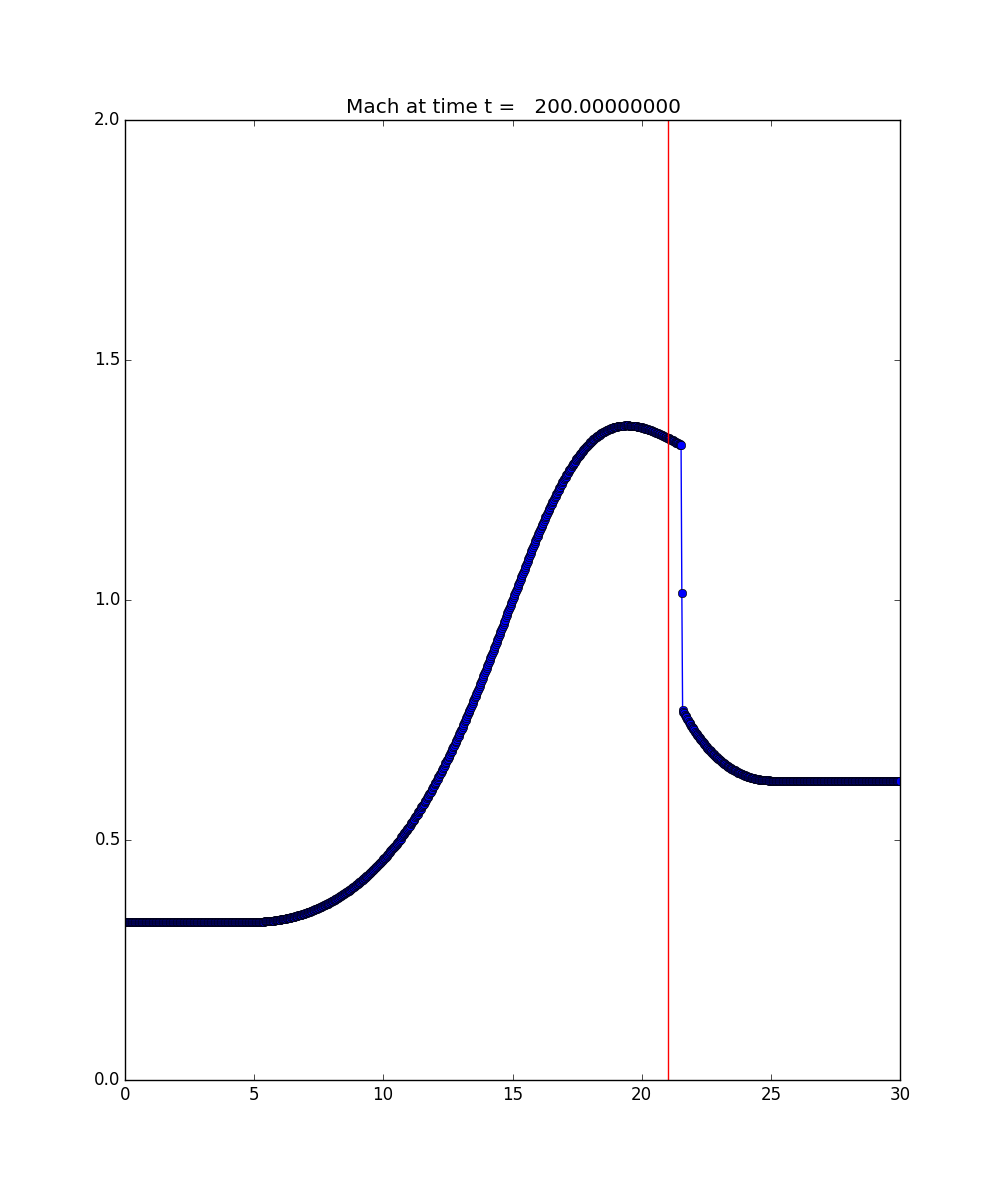
\includegraphics[height=6.5cm]{nozz2_045.png}}
\subfigure[$\frac{p_{atm}}{p_0}$ = 0.4]{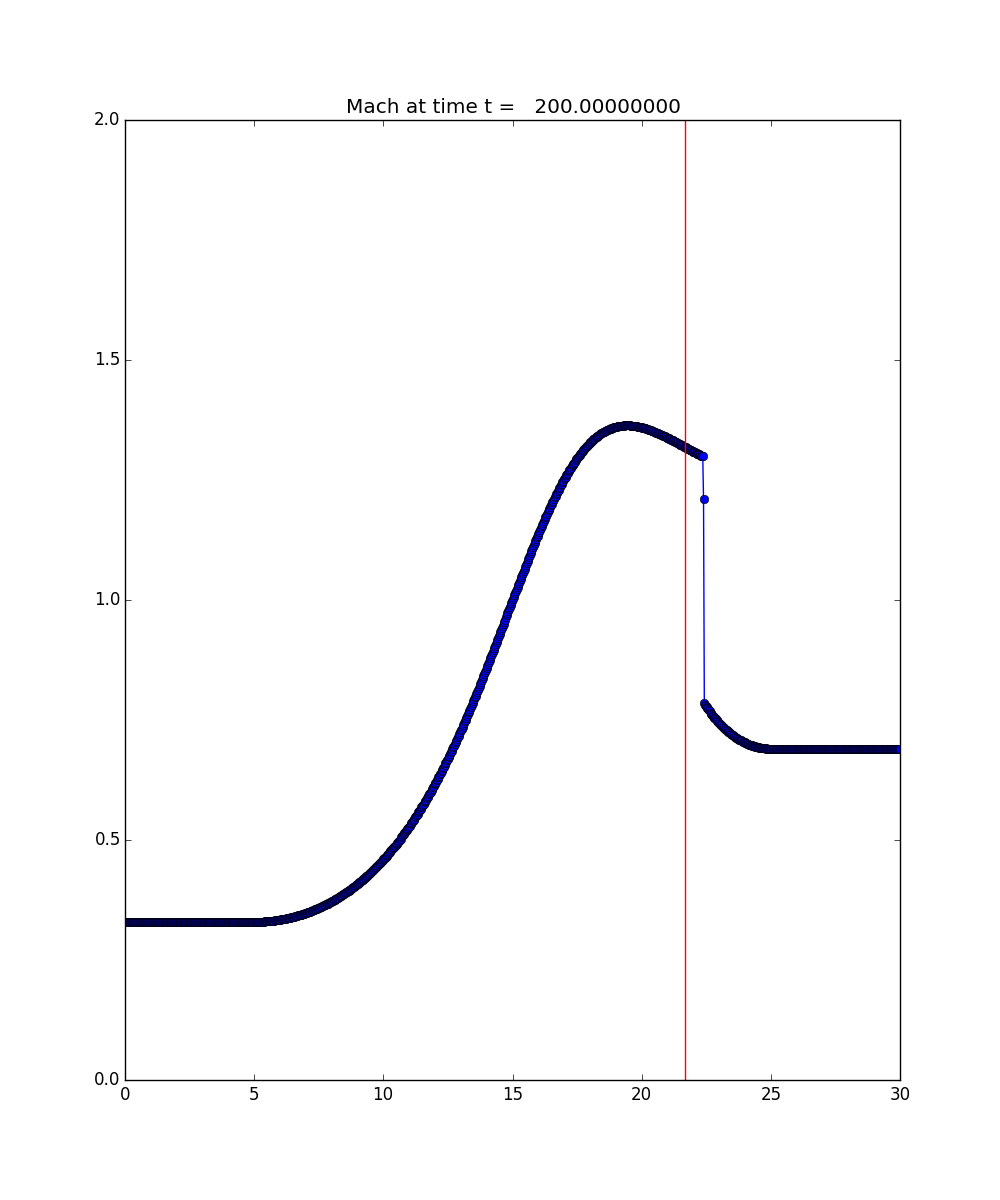
\includegraphics[height=6.5cm]{nozz2_04.png}}
\subfigure[$\frac{p_{atm}}{p_0}$ = 0.35]{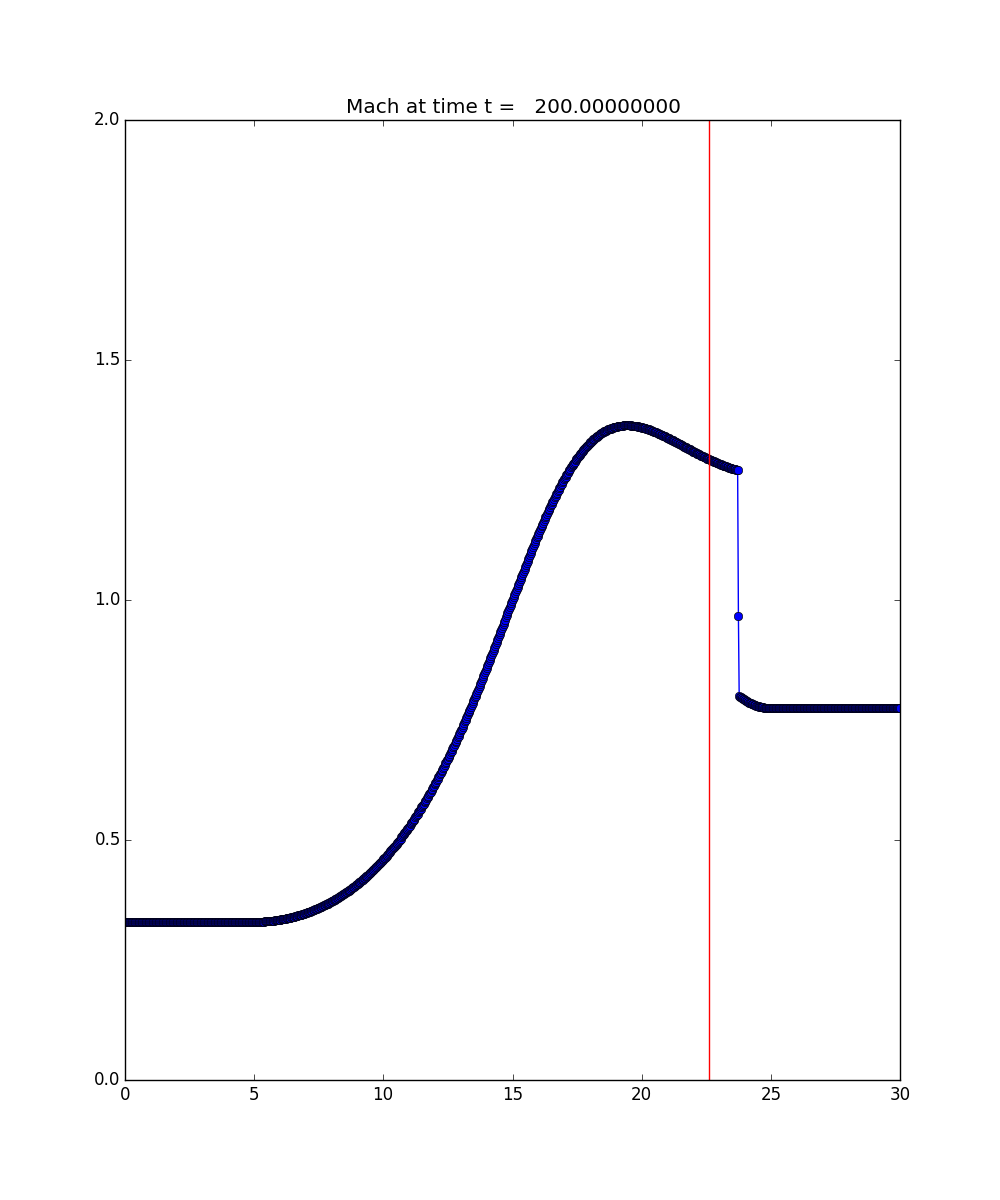
\includegraphics[height=6.5cm]{nozz2_035.png}}
\caption{Mach of Nozzle 2 at steady state for $\frac{p_{atm}}{p_0}$ = a). 0.45, b). 0.4, c). 0.35. As the pressure ratio decreases, the simulation shock deviates further from the theoretical shock location. \label{nozz2shock}}
\end{figure}

\section{Conclusion}
Overall, the results from Clawpack simulations were fairly consistent with theoretical shock locations, for higher pressure ratios when the shock was located away from the nozzle exit. At lower pressure ratios, simulations tended to diverge from expected results.

\pagebreak
\section*{References}
[1] Leveque, Randall J., Finite Volume Methods for Hyperbolic Problems, Cambridge University Press, New York, NY, 2011

[2] Liepmann, H.W. and Roshko, A., Elements of Gasdynamics, Dover Publications, Mineola, NY, 1985


\section*{Appendix}
\subsection*{Analytical Shock Location}

The theoretical shock location can be solved using isentropic relations, normal shock relations, and an iterative MATLAB code.

\begin{enumerate}
\item Guessing a shock location, $ x_s $ we can compute the area at the shock location $ A_s $.
\item 
Assuming choked flow at the throat, and a known area profile, the cross-sectional area at the throat $ A^* $ and a downstream area at the guessed shock location $ A_s $ are known. From this area ratio, the Mach just upstream of the shock, $ M_1 $ can be calculated using the isentropic area relation:
\begin{equation} \label{eq:isen}
\left( \frac{A_s}{A^*}\right)^2=\frac{1}{M_1^2} \left[ \frac{2}{\gamma +1} \left(1+\frac{\gamma-1}{2} M_1^2 \right) \right]^{\frac{\gamma+1}{\gamma-1}}
\end{equation}

\item Using a normal shock relation, we can calculate the Mach number $ M_2 $ just downstream of the shock:
\begin{equation}
M_2^2=\frac{1+\frac{\gamma-1}{2}M_1^2}{\gamma M_1^2-\frac{\gamma-1}{2}}
\end{equation}


\item From $ M_2 $, and $ A_s $, we can calculate a fictitious $ A^*_{exit} $ for some region downstream of the shock, using Eq. \ref{eq:isen}

\item Using Eq. \ref{eq:isen} with $ A^*_{exit} $ and the known area at the exit $ A_{exit} $ , we can calculate the Mach number at the exit, $ M_{exit} $, which should be a subsonic value.

\item We now need to compare the computed ratio of exit pressure to entrance pressure to the given pressure ratio. This is done through a product of pressure ratios, using isentropic and normal shock pressure relations.

In general, for any point in the flow:
\begin{equation} \label{eq:pt}
\frac{p_t}{p}=\left(1+\frac{\gamma-1}{2}M^2\right)^{\frac{\gamma}{\gamma-1}}
\end{equation}
Additionally, between any two points in a flow, total pressure remains constant, assuming isentropic flow, unless there is a shock, given by:
\begin{equation}
p_{1t}=p_{2t}
\end{equation}
In the case of a shock, the normal shock relation for two points on either side of the shock is given by:

\begin{equation} \label{eq:shock}
\frac{p_2}{p_1}=1+\left(\frac{2\gamma}{\gamma+1}(M_1^2-1)\right)
\end{equation}

We wish to solve for the pressure ratio $ p_{exit}/p_{in}=1.931 $ using the product of pressure ratios:

\begin{equation}
\frac{p_{exit}}{p_{in}}=
\underbrace{\frac{p_{exit}}{p_{exit,t}}}_{Eq. \ref{eq:pt}} \underbrace{\frac{p_{exit,t}}{p_{2,t}}}_{1}
\underbrace{\frac{p_{2,t}}{p_{2}}}_{Eq. \ref{eq:pt}}
\underbrace{\frac{p_{2}}{p_{1}}}_{Eq. \ref{eq:shock}}
\underbrace{\frac{p_{1}}{p_{1,t}}}_{Eq. \ref{eq:pt}}
\underbrace{\frac{p_{1,t}}{p_{in,t}}}_{1}
\underbrace{\frac{p_{in,t}}{p_{in}}}_{Eq. \ref{eq:pt}}
\end{equation}

\begin{equation}
\frac{p_{exit}}{p_{in}}=
\underbrace{\frac{p_{exit}}{p_{exit,t}}}_{isen} \underbrace{\frac{p_{exit,t}}{p_{2,t}}}_{1}
\underbrace{\frac{p_{2,t}}{p_{2}}}_{isen}
\underbrace{\frac{p_{2}}{p_{1}}}_{shock}
\underbrace{\frac{p_{1}}{p_{1,t}}}_{isen}
\underbrace{\frac{p_{1,t}}{p_{in,t}}}_{1}
\underbrace{\frac{p_{in,t}}{p_{in}}}_{isen}
\end{equation}

In the last pressure ratio $ \frac{p_{in,t}}{p_{in}} $ , $ M_{inlet} $ is set to 0.
\item If this pressure ratio was larger than the prescribed pressure ratio, the new guess for  $ x_s $ was increased by the MATLAB assignment $ x_s=x_s+0.01 $. Conversely, if the pressure ratio was lower than the pressure ratio, the new guess for  $ x_s $ was decreased by the MATLAB assignment $ x_s=x_s-0.01 $. This process was iterated in a loop until convergence.
\end{enumerate}
\end{document}
